\chapter{État de l'art}
\label{chap:etatdelart}

Une interface frictionnelle est formée par le contact de deux solides le long d'un plan. Lorsqu'elle est pressée et cisaillée, elle résiste au cisaillement et accumule de l'énergie élastique. Elle reste bloquée jusqu'à sa mise en mouvement soudaine au cours d'un évènement de glissement rapide (Sec.\,\ref{sec:frot}). Cette mise en glissement est médiée par une rupture interfaciale, brisant les microcontacts retenant le glissement entre les deux solides (Sec.\,\ref{sec:LEFM}). La rupture se propage jusqu'à la vitesse du son et initie, pour un système de taille finie, le mouvement de glissement macroscopique, qui ne peut avoir lieu qu'une fois que la totalité de l'interface s'est brisée. Ainsi chaque évènement de slip débute par une rupture. Ce cycle de stick-slip est caractéristique des interfaces frictionnelles, et est responsable des mouvements sismiques\,\cite{brace_stick-slip_1966}, décrits par la mécanique des failles (Sec.\,\ref{sec:failles}). Cependant les failles sismiques étant des systèmes mécaniques complexes, d'autres dynamiques en émergent, telles que des mouvements de glissement lent et des couplages dits \textit{co-sismiques}.

Notre étude a pour but de caractériser les mécanismes par lesquels la dynamique d'une interface frictionnelle modèle est modifiée par l'ajout de complexité dans le système. Nous nous intéressons particulièrement à une situation dans laquelle le contact entre les deux solides est perturbé par la présence d'un milieu granulaire. Cette situation est une modélisation minimaliste du contact frictionnel entre des roches au sein de failles tectoniques comportant une couche de gouge, milieu granulaire composé de roche broyée non cohésive. Notre étude se place donc à la croisée de plusieurs domaines de recherche actifs, s'intéressant à des systèmes d'échelles variées et utilisant des méthodes et approches parfois très différentes.


Nous présentons au cours de cette thèse un dispositif expérimental de cisaillement d'interfaces frictionnelles bidimensionnelles. Nous l'utilisons sur une interface frictionnelle composée par deux plaques minces de PMMA perturbée par la présence d'un patch de milieu granulaire dense ou d'une couche homogène de milieu granulaire. Ces interfaces sont respectivement une interface frictionnelle hétérogène pour laquelle le patch granulaire se comporte comme une zone en glissement lent, et une interface homogène granulaire. Nous mettons en évidence l'existence dans ces systèmes de ruptures dynamiques similaires à celles observées le long les interfaces solide-solide homogènes, mais également des comportements nouveaux, émergeant de la présence du milieu granulaire, et en particulier une déstabilisation de l'interface par le patch glissant. Dans ce chapitre, nous présentons un aperçu non exhaustif des connaissances publiées portant sur des thématiques connexes à ces problématiques. Tout d'abord, nous effectuons un récapitulatif de la dynamique d'une interface solide-solide homogène, décrite par la mécanique de la fracture linéaire élastique. Nous présentons ensuite les différents effets que peut avoir une hétérogénéité à l'interface sur cette dynamique. Enfin nous discutons des particularités des interfaces entièrement granulaires et de leurs descriptions dans la littérature.



\newpage

\minitoc

\newpage


\section{Dynamique d'une interface solide-solide homogène}

Une interface solide-solide homogène est composée de deux blocs solides macroscopiquement lisses, mis en contact, pressés et cisaillés. La dynamique macroscopique de ce type d'interface est un mouvement de stick-slip, dont l'initiation est médiée par une rupture fragile. Il a été montré que cette rupture est décrite par la mécanique de la fracture linéaire élastique (LEFM). Nous présentons dans cette section les dispositifs expérimentaux utilisés pour étudier ces interfaces, les observations des fractures qui s'y propagent, et la description de ces fractures par la théorie LEFM.

\subsection{Dispositifs expérimentaux utilisés}

Les dispositifs expérimentaux utilisés sont divers mais reposent sur le même principe. Une presse permet la compression et le cisaillement de deux blocs solides, tandis qu'un dispositif de mesure à haute fréquence permet de caractériser la propagation des ruptures. Nous détaillons ici quelques-uns de ces dispositifs.


\subsubsection{Presse mécanique}

\begin{figure}[htb]
\centering
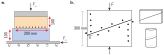
\includegraphics[scale=1]{../Figures_chap_etat/dispxp.pdf}
\caption[Deux types de presses mécaniques]{Schéma des deux méthodes d'application des forces normale et cisaillante. \textbf{a.}\,Application de la force cisaillante indépendamment de la force normale. La force normale est fixée, et la force cisaillante est pilotée par le déplacement du chariot (adapté de\,\cite{svetlizky_brittle_2019}). Dans le cas présent les carrés noirs symbolisent la position de jauges de déformation. \textbf{b.}\,Application d'une force unique sur une interface biseautée. L'angle du biseau $\alpha$ détermine la proportion de la force $F$ distribuée sur la normale et la tangente à l'interface (adapté de\,\cite{schubnel_photo-acoustic_2011}). Dans le cas présent les carrés noirs représentent la position de capteurs acoustiques et accélérométriques. Cette méthode d'application des forces peut être utilisée sur des plaques minces\,\cite{xia_laboratory_2004, nielsen_experimental_2010,mclaskey_foreshocks_2013, rubino_understanding_2017} ou sur des cylindres\,\cite{schubnel_photo-acoustic_2011,passelegue_sub-rayleigh_2013,passelegue_dynamic_2016}.}
\label{fig:dispxp}
\end{figure}

La presse mécanique a pour but de presser et cisailler les deux échantillons. Deux approches principales ont été mises en place. La première consiste en l'application d'une pression normale indépendamment de la force cisaillante, au moyen d'une presse purement normale et d'une platine de translation liée à l'extrémité d'un des blocs, tandis que l'autre est immobile\,\cite{rubinstein_detachment_2004,rubinstein_crack-like_2006,rubinstein_dynamics_2007,kammer_propagation_2012,kammer_slip_2014, svetlizky_classical_2014,svetlizky_brittle_2017,bayart_slippery_2016,svetlizky_brittle_2019} (Fig.\,\ref{fig:dispxp}a). Une variation de ce dispositif consiste en l'application de la force cisaillante directement sur le côté du bloc, dans toute sa hauteur\,\cite{rosakis_intersonic_2000,mclaskey_earthquake_2019}. La deuxième approche consiste en l'application d'une seule force sur les échantillons, sur une interface effectuant un angle relativement à cette force\,\cite{xia_laboratory_2004,nielsen_experimental_2010, schubnel_photo-acoustic_2011, latour_characterization_2013, mclaskey_foreshocks_2013, passelegue_sub-rayleigh_2013, passelegue_dynamic_2016,rubino_understanding_2017} (Fig.\,\ref{fig:dispxp}b). L'angle choisi est alors pris proche de l'angle critique pour lequel le mouvement de stick-slip peut avoir lieu, c'est à dire $\alpha_c =\arctan \mu_s$.



\subsubsection{Échantillons pressés}

Les échantillons choisis sont presque systématiquement des plaques minces, et occasionnellement des cylindres (études menées dans le groupe de F.\,X.\,Passelègue). Ce choix permet d'effectuer une hypothèse de planéité des contraintes, et donc de réduire le système étudié à deux dimensions. L'interface formée par ces plaques peut alors varier en longueur de l'ordre de quelques centimètres pour la plupart des études jusqu'à un ou plusieurs mètres (études menées dans les groupes de E.\,Fukuyama et G.\,C.\,McLaskey).

Les matériaux choisis diffèrent selon les études. Lorsque la portée de l'étude considérée est orientée vers la géophysique ou la mécanique des roches, ce sont des échantillons de roches qui sont choisis, comme par exemple du granite (études menées dans les groupes de E.\,Fukuyama, G.\,C.\,McLaskey et A.\,Schubnel).
%Ces roches ont cependant des inconvénients dans le cadre d'expériences nécessitant des propriétés mécaniques et optiques spécifiques. Pour cela des matières plastiques sont utilisées.
L'utilisation de roches présente cependant plusieurs inconvénients, tels que la grande vitesse de propagation des ondes acoustiques en leur sein ou les possibles hétérogénéités des échantillons.
Des matières plastiques sont utilisées afin de réduire la vitesse des ondes dans le milieu et d'assurer l'homogénéité de l'échantillon utilisé. Leur transparence permet également d'implémenter des mesures à l'interface par imagerie.
Deux catégories de plastiques polymères ressortent, les plastiques acryliques tels que le PMMA (études menées dans le groupe de J.\,Fineberg)\,\cite{rubinstein_detachment_2004,rubinstein_crack-like_2006,rubinstein_dynamics_2007, svetlizky_classical_2014,svetlizky_brittle_2017, bayart_slippery_2016, svetlizky_brittle_2019} et les plastiques polycarbonates tels que le PADC (homalite, études menées dans les groupes de A.\,J.\,Rosakis et A.\,Schubnel)\,\cite{rosakis_intersonic_2000, xia_laboratory_2004, latour_characterization_2013, nielsen_experimental_2010, schubnel_photo-acoustic_2011, rubino_understanding_2017}. Ces deux familles de matériaux ont des propriétés mécaniques proches, avec notamment un module d'Young de quelques gigapascals (contre plusieurs dizaines de gigapascals pour les roches).


En fonction des propriétés mécaniques et optiques des matériaux, plusieurs techniques de mesure sont implémentées sur ces systèmes.

\subsubsection{Dispositifs de mesure}


Les dispositifs de mesure utilisés pour déterminer les contraintes  à l'interface et mesurer la propagation de ruptures sont répartis en trois catégories (Fig.\,\ref{fig:dispmes}).

Tout d'abord les mesures peuvent être des mesures directes du tenseur des déformations sur les surfaces des échantillons, au moyen de jauges de déformation (études menées dans les groupes de J.\,Fineberg, G.\,C.\,McLaskey, A.\,Schubnel et M.\,Violay).
%\,\cite{rubinstein_detachment_2004,rubinstein_crack-like_2006,rubinstein_dynamics_2007,kammer_propagation_2012,kammer_slip_2014, svetlizky_classical_2014, svetlizky_brittle_2017, bayart_slippery_2016, svetlizky_brittle_2019, mclaskey_stress_2011, mclaskey_slow_2017}
Ces mesures permettent de déterminer directement le tenseur des déformations dans le bloc grâce à l'hypothèse de planéité des contraintes permise par leur géométrie.
%Elles nécessitent un dispositif d'acquisition électronique rapide doublé d'un système d'amplification électronique à faible bruit.

La transparence des matériaux plastiques permet d'utiliser des méthodes de mesure optique en imageant l'interface ou la surface des blocs au moyen d'une caméra rapide. L'interface peut être imagée par réflexion interne totale (TIR) afin de mesurer en temps réel la surface de contact réelle $A_r$ entre les deux blocs (études menées dans les groupes de J.\,Fineberg et G.\,C.\,McLaskey, Fig.\,\ref{fig:dispmes}a).
%\,\cite{rubinstein_detachment_2004,rubinstein_crack-like_2006,rubinstein_dynamics_2007,kammer_propagation_2012,kammer_slip_2014, svetlizky_classical_2014,svetlizky_brittle_2017,bayart_slippery_2016,svetlizky_brittle_2019}
Les propriétés photoélastiques du PADC pour leur part permettent de mesurer les déformations des blocs par les changements d'indice optique en transmission (études menées dans les groupes de S.\,Latour, S.\,Nielsen et A.\,J.\,Rosakis, Fig.\,\ref{fig:dispmes}).
%\,\cite{rosakis_intersonic_2000, xia_laboratory_2004}
D'autres mesures optiques sont possibles, telles que la mesure des déformations à la surface d'un bloc par des méthodes de corrélation d'images (DIC, études menées par les groupes de N.\,Lapusta et A.\,J.\,Rosakis)\,\cite{rubino_understanding_2017,buijze_nucleation_2020}. Il est enfin possible d'effectuer des mesures acoustiques des ondes se propageant dans le matériau
%\,\cite{nielsen_experimental_2010,schubnel_photo-acoustic_2011, passelegue_sub-rayleigh_2013}
(études menées dans le groupe de A.\,Schubnel, Fig.\,\ref{fig:dispmes}c). Ces mesures proches des mesures sismologiques permettent de déterminer la vitesse de propagation d'une rupture ou la position de l'épicentre d'un évènement grâce au contenu fréquentiel et au retard des ondes acoustiques émises.


Ces mesures diverses convergent vers un résultat similaire, qui est l'observation de la propagation de ruptures à l'interface frictionnelle.




\begin{figure}[p!]
\centering
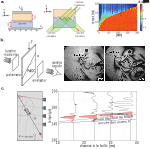
\includegraphics[scale=1]{../Figures_chap_etat/dispmes.pdf}
\caption[Présentations des différentes mesures]{Différentes méthodes de mesure de la propagation de rupture à l'interface. \textbf{a.}\,Mesure optique de la surface de contact réelle par réflexion interne totale.  (adapté de\,\cite{svetlizky_brittle_2019}). Deux plaques de PMMA sont pressées ($F_N=\SI{5500}{\newton}$) et cisaillées. Une réduction rapide de $A(x, t)$ a lieu au moment d'une chute de force cisaillante. La fracture se propage de gauche à droite, le temps est en ordonnée. Les portions d'interface dans lesquelles la fracture est déjà passée ont une aire de contact plus faible (bleu) que les régions encore intactes (rouge) \textbf{b.}\,Mesure optique des déformations par photoélasticimétrie dans un bloc de PADC au passage d'une rupture sub-Rayleigh (gauche) et supershear (droite) (adapté de\,\cite{xia_laboratory_2004}). Les déformations des plaques modifient l'indice optique extraordinaire $n_e$ de la plaque biréfringente, entraînant des variations de polarisation de la lumière. \textbf{c.}\,Mesure acoustique de la propagation d'une rupture (adapté de\,\cite{passelegue_sub-rayleigh_2013}). L'arrivée des ondes de compression sur les détecteurs permet de repérer l'avancée de la rupture. Dans le cas d'une rupture supershear, la même mesure peut s'effectuer par la détection du cône de Mach associé.}
\label{fig:dispmes}
\end{figure}

\subsection{Ruptures interfaciales}

\subsubsection{Observation des ruptures}



Au moyen des méthodes décrites ci-dessus, les études précédemment citées montrent que l'initiation d'un mouvement de glissement rapide au cours d'un cycle de stick-slip s'accompagne de la propagation d'une rupture dynamique à l'interface. Cette rupture consiste en l'affaiblissement des contacts frictionnels entre les blocs, comme montré par la réduction de la surface de contact réelle $A_r$ au moment de l'initiation du mouvement\,\cite{svetlizky_brittle_2019}. Il a été montré que ces ruptures peuvent être séparées en deux catégories en fonction de leur vitesse $v$. Les ruptures telles que $v<c_r$ la vitesse des ondes de Rayleigh dans le matériau considéré sont dites sub-Rayleigh. D'autres ruptures telles que $v>c_s$ la vitesse des ondes de cisaillement dans le matériau sont observées. Ces ruptures sont dites supershear, et du fait de leur vitesse supérieure à la vitesse des ondes dans le milieu, elles sont accompagnées d'un cône de Mach. Ces deux types de ruptures peuvent interagir, des études montrent en particulier qu'une rupture sub-Rayleigh peut déclencher une rupture supershear\,\cite{xia_laboratory_2004, schubnel_photo-acoustic_2011,passelegue_sub-rayleigh_2013}. La vitesse de ces ruptures est contrôlée par l'énergie élastique disponible au moment de leur initiation\,\cite{svetlizky_brittle_2017}.




\subsubsection{Simulation des ruptures}


La propagation de ruptures à l'interface frictionnelle a également été observée dans des simulations numériques de dispositifs similaires ou de systèmes minimaux\,\cite{radiguet_survival_2013, barras_study_2014, tromborg_slow_2014, amundsen_steady-state_2015, thogersen_minimal_2019}. Ces modèles permettent de rendre compte des phénomènes observés dans les systèmes expérimentaux décrits ci-dessus, comme la transition entre une rupture sub-Rayleigh et supershear\,\cite{passelegue_sub-rayleigh_2013,kammer_equation_2018, svetlizky_dynamic_2020}, mais également de phénomènes plus complexes tels que la robustesse de cette phénoménologie dans le cas d'interfaces formées par deux blocs de matériaux différents\,\cite{barras_study_2014,bar-sinai_slow_2012}.


\subsubsection{Description quantitative des ruptures}



\begin{figure}[htb]
\centering
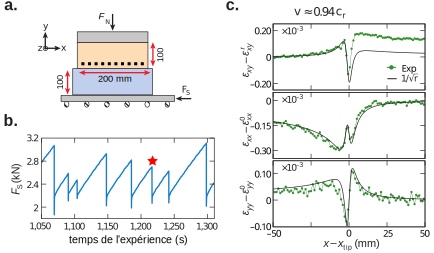
\includegraphics[scale=1]{../Figures_chap_etat/svet_propag.pdf}
\caption[Mesure des déformations associées à une rupture frictionnelle]{Mesure des déformations associées à une rupture frictionnelle (adapté de\,\cite{svetlizky_brittle_2019}). \textbf{a.}\,Dispositif expérimental. Deux plaques de PMMA ($c_r \simeq \SI{1250}{\meter\per\second}$) sont pressées l'une contre l'autre avec une force normale $F_N=\SI{5500}{\newton}$. \textbf{b.}\,L'interface subit un mouvement de stick-slip lorsque la force cisaillante $F_S$ augmente de manière quasi-statique. \textbf{c.}\,Mesures des variations du tenseur des déformations lors de l'évènement marqué d'une étoile rouge. Les prédictions LEFM sont tracées en noir, $\Gamma\simeq\SI{2.5}{\joule\per\meter\squared}$ est le seul paramètre libre.}
\label{fig:reflex}
\end{figure}


Dans le cas des ruptures sub-Rayleigh, il a été montré que les déformations qu'elles engendrent ainsi que leur propagation sont décrites par la mécanique de la fracture linéaire élastique (LEFM)\,\cite{kammer_linear_2015,svetlizky_brittle_2019} (Fig.\,\ref{fig:reflex}). La mesure des déformations à l'aide de jauges de déformation montre qu'au passage d'une rupture à l'interface, $\varepsilon_{xy}$ décroît d'une valeur initiale $\varepsilon_{xy}^0$ à $\varepsilon_{r}$, en effectuant une vaguelette (Fig.\,\ref{fig:reflex}). Cette vaguelette est caractéristique des ruptures LEFM, décrites par l'Équation\,\ref{eq:fracdynfric} pour un crack en mode\:\textsc{ii}. Il est notamment possible d'effectuer un ajustement du signal mesuré par les prédictions théoriques, avec pour seul paramètre libre l'énergie de fracture, ce qui donne un excellent accord. La dynamique des ruptures ainsi observées est également décrite par les équations de la théorie LEFM\,\cite{svetlizky_brittle_2017}.



Nous avons vu dans cette section que la caractérisation de la dynamique d'une interface frictionnelle solide-solide est bien comprise. Il est attesté que le mouvement de glissement s'amorce par le moyen de la propagation d'une rupture frictionnelle, aussi bien dans les matériaux plastiques que dans les roches. Cette rupture peut être mesurée par des techniques optiques, électromécaniques ou acoustiques. Dans le cas des ruptures sub-Rayleigh, il est même possible de la décrire au moyen de la théorie LEFM.


Les interfaces frictionnelles d'intérêt géologique sont cependant complexes de part leur géométrie, leur composition, et leur histoire, les menant à incorporer des hétérogénéités.


\section{Interface hétérogène}
\label{sec:hetero}


Nous appelons interface hétérogène une interface comportant dans sa longueur une hétérogénéité locale. Cette hétérogénéité peut consister en une différence de composition, par exemple la présence d'un patch de lubrifiant, de milieu granulaire, ou d'un matériau différent. Elle peut également consister en une altération mécanique ou géométrique de la surface de contact, comme la présence d'un trou, d'un état de surface différent, ou d'un défaut ou excès de chargement local. Les failles sismiques réelles sont hautement hétérogènes, et l'étude en laboratoire et la simulation d'hétérogénéités modèles permettent d'améliorer leur compréhension.

Nous présentons dans cette section les modifications de la dynamique d'une interface frictionnelle dues à la présence d'une hétérogénéité. Celle-ci peut agir comme une barrière à la propagation d'une rupture interfaciale ou comme une zone de glissement lent.





\subsection{L'hétérogénéité agit comme une barrière}
La propagation d'une rupture observée sur une portion d'interface peut ralentir ou s'arrêter à la rencontre de l'hétérogénéité. Ce phénomène est considéré comme pouvant être à l'origine de l'arrêt des séismes.

\subsubsection{Mécanismes d'arrêt}

\begin{figure}[htb]
\centering
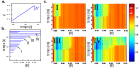
\includegraphics[scale=0.9]{../Figures_chap_etat/arrested.pdf}
\caption[Ruptures arrêtées]{Ruptures arrêtées par une inhomogénéité de contrainte, et donc d'énergie de rupture (adapté de\,\cite{rubinstein_dynamics_2007}). \textbf{a.}\,Mouvement de stick-slip à l'interface. \textbf{b.}\,Longueur des évènements de rupture. Les évènements I, II et III sont des ruptures arrêtées, tandis que l'évènement IV est une rupture traversant toute l'interface. \textbf{c.}\,Aire réelle de contact normalisée au cours des quatre évènements repérés. La faible aire de contact à l'extrémité gauche de l'interface correspond à une zone de faible énergie de fracture.}
\label{fig:moche}
\end{figure}





% La raison de l'arrêt de la propagation d'une rupture est le changement d'énergie de fracture. En effet si $\Gamma$ dépend de la position le long de l'interface, la propagation du crack ne s'effectue pas à vitesse constante (Éq.\,\ref{eq:propagfracdyn}). Une rupture initiée dans une région où $\Gamma$ est faible peut perdre en vitesse puis s'arrêter dans une région où $\Gamma$ est plus élevé. La rupture peut également être déviée, ou guidée par d'autres plans faibles que le plan principal de l'interface\,\cite{gudmundsson_effects_2010}.

% Un exemple de rupture arrêtée apparaît lors de l'introduction de lubrifiant sur une portion seulement de l'interface\,\cite{bayart_slippery_2016, bayart_rupture_2018}. Lorsqu'une rupture nuclée dans une portion de l'interface sans lubrifiant, elle peut être stoppée par la zone lubrifiée en raison de l'augmentation d'énergie de fracture qu'elle rencontre. En effet le critère de propagation $G=\Gamma$ (Éq.\,\ref{eq:propagfracdyn}) n'est plus vérifié en cas de changement soudain de $\Gamma$ à l'interface.



% La même phénoménologie apparaît lorsque la contrainte cisaillante appliquée n'est pas spatialement homogène (Éq.\,\ref{eq:homospa}), les fronts de rupture peuvent se propager sur une portion de l'interface et s'arrêter avant de briser l'ensemble de l'interface\,\cite{kammer_linear_2015,
%radiguet_survival_2013,
%rubinstein_dynamics_2007,
%scheibert_role_2010,
%bayart_rupture_2018,
%taloni_scalar_2015}. Ainsi un défaut de chargement dans une interface frictionnelle solide-solide peut mener à l'apparition de ruptures arrêtées, comme montré par Bayart et al.\,\cite{bayart_slippery_2016} (Fig.\,\ref{fig:moche}).Ces ruptures partielles de l'interface sont des précurseurs d'un mouvement de glissement macroscopique de l'interface, comparables aux \textit{foreshocks} des séismes de grande magnitude.


%Les ruptures arrêtées agissent également comme des hétérogénéités de contraintes par la concentration des contraintes qu'elles occasionnent en leur point d'arrêt. Cette situation est particulièrement pertinente dans le cadre de la prévention sismique, puisque les séismes ne sont jamais des ruptures de toute la longueur d'un système de faille, mais des ruptures arrêtées.



Une rupture peut dans certains cas être arrêtée par un changement d'énergie de fracture. En effet si $\Gamma$ dépend de la position le long de l'interface, la propagation du crack ne s'effectue pas à vitesse constante (Éq.\,\ref{eq:propagfracdyn}). Une rupture initiée dans une région où $\Gamma$ est faible peut s'arrêter dans une région où $\Gamma$ est plus élevé, le critère de propagation $G=\Gamma$ n'étant alors plus vérifié. Un exemple de rupture arrêtée apparaît lors de l'introduction de lubrifiant sur une portion seulement de l'interface\,\cite{bayart_slippery_2016, bayart_rupture_2018}. Lorsqu'une rupture nuclée dans une portion de l'interface sans lubrifiant, elle peut être stoppée par la zone lubrifiée en raison de l'augmentation d'énergie de fracture qu'elle rencontre.


La même phénoménologie peut apparaître lorsque la contrainte cisaillante appliquée n'est pas spatialement homogène (Éq.\,\ref{eq:homospa}), les fronts de rupture s'arrêtant alors avant de briser l'ensemble de l'interface\,\cite{kammer_linear_2015,
radiguet_survival_2013,
rubinstein_dynamics_2007,
scheibert_role_2010,
bayart_rupture_2018,
taloni_scalar_2015}. Ainsi un défaut de chargement dans une interface frictionnelle solide-solide peut mener à l'apparition de ruptures arrêtées, comme montré par Bayart et al.\,\cite{bayart_fracture_2016} (Fig.\,\ref{fig:moche}). Ces ruptures partielles sont des précurseurs d'un mouvement de glissement macroscopique de l'interface, comparables aux \textit{foreshocks} des séismes de grande magnitude. Les ruptures arrêtées agissent également comme des hétérogénéités de contraintes par la concentration des contraintes qu'elles occasionnent en leur point d'arrêt. Cette situation est particulièrement pertinente dans le cadre de la prévention sismique, puisque les séismes ne sont jamais des ruptures de toute la longueur d'un système de faille, mais des ruptures arrêtées.

La dynamique de la rupture peut également être affectée par les propriétés géométriques de l'interface. Elle peut être arrêtée, déviée, ou guidée par d'autres plans faibles que le plan principal de l'interface\,\cite{gudmundsson_effects_2010}, ou par la présence d'un milieu granulaire.





\subsubsection{Barrière granulaire}


L'hétérogénéité menant à l'arrêt de la propagation peut également consister en une inclusion de milieu granulaire à l'interface\,\cite{rubino_intermittent_2022,buijze_nucleation_2020,buijze_effects_2021}. Le mécanisme par lequel une inclusion de milieu peu cohésif interagit avec les portions solide-solide de l'interface reste mal compris, et reste généralement expliqué par les descriptions empiriques des modèles Rate-and-State. Rubino et al. ont par exemple observé par DIC des ruptures s’arrêtant dans une couche de gouge localisée, et l'ont attribué au comportement renforcé en vitesse de la gouge\,\cite{rubino_intermittent_2022}. Cette description coïncide avec celle proposée par Buijze et al. d'une interface entièrement granulaire hétérogène\,\cite{buijze_nucleation_2020}. Cette phénoménologie rapprocherait alors le patch granulaire d'un patch glissant, que nous décrivons dans la section suivante.

L'hétérogénéité peut être artificiellement créée, mais même lorsque qu'un milieu granulaire est initialement réparti à l'interface de manière homogène, des hétérogénéités émergent. En effet la formation d'une hétérogénéité peut être imputée à l'usure 
de l'interface. Dans le cas d'une interface de roches séparées par une poudre fine et homogène, la répartition de la poudre peut changer jusqu'à former des hétérogénéités de contraintes\,\cite{cebry_creep_2022, buijze_nucleation_2020,gvirtzman_nucleation_2021}. Dans le cas de Cebry et al., le système étudié, une interface de blocs plastiques encapsulant une fine couche de poudre de quartz, a naturellement évolué vers la formation de deux aspérités. Ces deux aspérités imposent alors une dynamique complexe à l'interface, entraînant une co-sismicité de ses différentes portions.

\subsubsection{Co-sismicité}
La co-sismicité est la manifestation d'un couplage entre deux failles sismiques. Lorsqu'une faille se rompt dans un évènement sismique, les contraintes qu'elle retenait sont relâchées, et redistribuées aux failles avoisinantes. Cette co-sismicité se retrouve dans des systèmes pour lesquels la rupture arrêtée par l'hétérogénéité entraîne la nucléation d'une autre rupture de l'autre côté de l'hétérogénéité, l'arrêt de la rupture reportant les contraintes libérées par la partie brisée sur la portion encore intacte de l'interface\,\cite{rubino_intermittent_2022}. La rupture arrêtée est alors un précurseur pour un évènement de rupture de l’interface entière.

Ces phénomènes soulèvent la question des mécanismes de couplage entre les différentes portions d'une faille. Ces mécanismes sont importants dans la compréhension des phénomènes de précurseurs et répliques (\textit{foreshocks and aftershocks}) des séismes\,\cite{felzer_common_2004}, ces ruptures arrêtées pouvant alors être des précurseurs de séismes de magnitude plus élevée. Au contraire après un séisme la zone déchargée peut agir comme une hétérogénéité de contrainte pouvant arrêter une rupture sismique déclenchée dans une portion de faille voisine, limitant ainsi l'amplitude des répliques.


Une hétérogénéité arrêtant une rupture peut être décrite dans le cadre des modèles Rate-and-State par la présence dans une interface d'un patch dont la dépendance du frottement en vitesse est différente de celle du reste de la faille\,\cite{chen_scaling_2009,schwartz_slow_2007,noda_stable_2013} (Sec.\,\ref{sec:rateandstate}). Cette description suppose cependant que la portion renforcée de l'interface glisse lentement lorsqu'elle est soumise à une contrainte cisaillante extérieure. Nous présentons par la suite des systèmes dans lesquels des portions de failles ne présentent pas d'activité sismique et relâchent les contraintes par le moyen d'un glissement lent.



\subsection{L'hétérogénéité est une zone en glissement lent}



Certaines portions de failles sismiques sont en mouvement lent, soit permanent, soit ponctuel au cours d'évènements de quelques minutes ou plus\,\cite{peng_integrated_2010,burgmann_geophysics_2018}. Le mécanisme responsable de ces phases de glissement reste encore méconnu, tout comme son rôle dans l'activité sismique d'une zone de failles\,\cite{radiguet_triggering_2016,dragert_silent_2001}. Dans cette section nous présentons ces zones de glissement, qui sont des hétérogénéités au sein d'une interface frictionnelle bloquée par ailleurs.


\subsubsection{Observation du glissement lent}

Les séismes lents ont d'abord été observés dans les zones de subduction, en particulier au Japon, situé au-dessus d'une des zones sismiques les plus actives du monde\,\cite{kanamori_mechanism_1972}. Ces observations d'abord indirectes\,\cite{sacks_slow_1978} ont mené à les nommer également séismes silencieux (\textit{silent earthquakes}) en raison de la faiblesse de leurs émissions acoustiques. Des méthodes de mesure directe ont permis d'observer ce phénomène dans de nombreuses régions de failles\,\cite{harris_large_2017}. Les techniques d'observation modernes reposent principalement sur l'usage de données GPS, permettant un suivi précis au centimètre près du mouvement de la croûte terrestre.

Les zones de glissement lent sont surveillées de près par de nombreuses équipes de recherche. Une partie de la littérature actuelle portant sur ces séismes lents consiste en la description d'une région spécifique, généralement après ou avant un évènement sismique majeur. Par exemple Ozawa et al.\,\cite{ozawa_coseismic_2011} décrivent les répliques et précurseurs du grand séisme de Tōhoku de 2011, de magnitude $M_w=9$, mesurés par des données GPS. Ces résultats sont ensuite agrégés dans des études sur de longues périodes ou des méta-études telles que celle de Schwartz et Rokosky\,\cite{schwartz_slow_2007}, montrant que le glissement lent est un phénomène généralisé présent entre autres tout autour de la ceinture de feu du Pacifique. Il a de plus été observé que ces zones de glissement lent peuvent correspondre à des hétérogénéités de composition au sein d'un système de failles. Des mesures par carottage dans certaines failles en glissement lent particulièrement peu profondes au large de la Nouvelle Zélande montrent notamment que les séismes lents sont induits par des régions de forte hétérogénéité mécanique, frictionnelle, pétrographiques et géométrique\,\cite{barnes_slow_2020}. Une hétérogénéité de composition peut se traduire par une hétérogénéité dans la dynamique de la faille.

Ainsi les zones de glissement sont extensivement observées, décrites et étudiées, pourtant Schwartz et Rokosky indiquent que malgré cette profusion d'études, les mécanismes à l'origine de leur glissement et leur influence sur les zones de failles bloquées «\,\textit{restent élusifs}\,». Ils sont souvent passés sous silence au profit d'une approche plus empirique basée sur des modèles Rate-and-State (Sec.\,\ref{sec:rateandstate}), dont les coefficients sont ajustés pour décrire des portions de failles spécifiques. L'étude en laboratoire de failles en glissement lent, au travers des expériences telles que celle que nous présentons dans cette thèse (Chap.\,\ref{sec:chaparticle}) ou de simulations numériques, permet d’améliorer notre compréhension de ces mécanismes, mais également des interactions entre les différentes portions d'un système de failles.



\subsubsection{Modélisation des failles glissantes}

\begin{figure}[htb]
\centering
\includegraphics[scale=1]{../Figures_chap_etat/buijze.pdf}
\caption[Effet d'une gouge hétérogène sur le stick-slip]{Mouvement de stick-slip au sein d'une interface comportant une gouge hétérogène cisaillée (extrait de\,\cite{buijze_effects_2021}). La gouge est pressée à une contrainte normale $\sigma_2$, et cisaillée à une contrainte $\tau^*$. L'hétérogénéité est constituée d'un patch de composition minéralogique différente pour chaque couleur de courbe. En orange la gouge est homogène. Les courbes bleue, verte et rouge correspondent à trois compositions différentes pour l'hétérogénéité. Le mouvement de stick-slip peut, en fonction de l'hétérogénéité choisie, disparaître, s'accélérer ou ponctuer un glissement permanent.}
\label{fig:buijze}
\end{figure}



La conception de failles sismiques en laboratoire permet de contrôler avec précision les propriétés des matériaux insérés à l'interface, et d'étudier les variations dans la dynamique de celle-ci avec les propriétés de l'hétérogénéité insérée\,\cite{bedford_fault_2022,buijze_effects_2021,kaproth_slow_2013}. Buijze et al. ont en particulier étudié l'influence d'une hétérogénéité pétrographique au sein d'une gouge pressée entre deux blocs de PMMA\,\cite{buijze_effects_2021}. La faille de laboratoire a alors exhibé une grande variété de dynamiques selon la gouge utilisée. Les exemples notables sont un mouvement de stick-slip particulièrement bien défini (Fig.\,\ref{fig:buijze}, courbe orange), et au contraire une mise en glissement permanent de l'interface toute entière (courbe bleue). L'hétérogénéité locale est alors responsable de la mise en glissement lent de toute l'interface.

Bedford et al. pour leur part montrent que l'insertion d'une gouge d'argile et de quartz à l'interface entre deux blocs de roche cisaillés mène à l'apparition, en fonction de la proportion d'argile ou de sa disposition, soit d'une instabilité de stick-slip, soit d'une mise en glissement lent\,\cite{bedford_fault_2022}. L'augmentation de la proportion d'argile entraîne un renforcement en vitesse de l'interface.



Ainsi une hétérogénéité locale à l'interface peut agir comme un patch glissant, menant à une modification de la dynamique globale de l'interface. Ce glissement lent est généralement étudié sous le prisme des modèles Rate-and-State. Cette analyse, bien qu'elle passe sous silence les mécanismes responsables du glissement, permet la modélisation d'un système de failles par un patchwork de zones dont les coefficients $A$ et $B$ sont choisis pour représenter des systèmes réels ou modèles, dans l'objectif de déterminer l'influence de ce patchwork sur la sismicité globale de la région d'intérêt.


\subsubsection{Rôle sismologique du glissement lent}

Les systèmes de failles sismiques sont fortement couplés. La rupture d'une portion de faille influence la dynamique de toute la faille par {co-sismicité}. Ainsi il a été montré que le glissement lent d'une portion de faille peut déclencher une rupture sismique\,\cite{radiguet_triggering_2016}, et inversement une rupture sismique peut débloquer des portions de failles avoisinantes, se mettant en glissement lent\,\cite{ozawa_coseismic_2011,chlieh_coseismic_2007}. Ce dernier mécanisme est adjacent à celui de l'apparition de répliques, séismes déclenchés par un premier évènement de rupture, généralement de plus faible magnitude que celui-ci.


Afin de décrire ces phénomènes des modèles Rate-and-State sont utilisés. De nombreuses simulations montrent que les portions de failles en glissement lent ont un rôle déterminant dans le comportement des failles\,\cite{lui_repeating_2016,noda_stable_2013,harris_large_2017,radiguet_survival_2013,chen_scaling_2009, romanet_fast_2018}. Lorsque ces simulations sont axées vers la description d'un système de failles réel, l'ajustement des paramètres $A$ et $B$ des portions de failles définies est un facteur clé de l'étude. Noda et Lapusta\,\cite{noda_stable_2013} montrent notamment en modélisant la zone de faille de Fukushima au Japon que le glissement lent de certaines portions de faille mène à la déstabilisation de portions pourtant théoriquement stables, car stabilisées par la vitesse. Chen et Lapusta\,\cite{chen_scaling_2009} effectuent une étude similaire en partant des propriétés d'une portion de la faille de San Andreas. Les implications de ces études vont pourtant au-delà de la description d'un système de failles précis.

Des simulations plus générales permettent d'étudier la co-sismicité dans des systèmes modèles, et d'en comprendre les mécanismes. Il a ainsi été montré que les transferts d'énergie élastique dans les failles modèles peuvent s'effectuer à grande distance, de l'ordre de \SI{600}{\kilo\meter} le long de la faille de San Andreas entre San Francisco et Los Angeles par exemple\,\cite{lui_repeating_2016}. À la recherche de la complexité minimale nécessaire à l’apparition de ces phénomènes, il a également été montré que la présence d'une hétérogénéité n'est pas nécessaire à l'émergence d'un tel couplage au sein de failles modèles, qui peut être déclenché par des effets géométriques\,\cite{romanet_fast_2018,liu_aseismic_2005}.


L'influence d'une hétérogénéité à l'interface sur le comportement macroscopique de celle-ci est due à la création d'une zone en glissement lent au sein de la faille. Cette zone agit comme une barrière à la propagation des ruptures, mais n'isole pas pour autant les portions de failles de part et d'autre du patch glissant. Au contraire la présence de ces hétérogénéités est responsable de phénomènes de co-sismicité et d'interactions à longue portée au sein de systèmes de failles.

Au cours de cette section nous avons présenté des hétérogénéités de composition formées par des milieux granulaires hétérogènes, la section suivante présente des études portant sur les interfaces frictionnelles entièrement granulaires homogènes.



\section{Interface entièrement granulaire homogène}

L'hétérogénéité d'une l'interface peut être médiée par l'insertion d'une couche de gouge entre deux blocs solides. La gouge est une roche broyée non cohésive située au cœur des failles, façonnée par l'usure des matériaux en contact cisaillant. Ses propriétés mécaniques sont celles d'un milieu granulaire très polydisperse, pressé et cisaillé par la roche. L'influence d'un tel milieu granulaire sur la dynamique d'une interface frictionnelle peut être étudiée en laboratoire grâce à l'utilisation de milieu granulaires modèles, pressés et cisaillés par des matériaux solides.


\subsection{Rhéologie granulaire}



Les expériences de rhéologie granulaire se focalisent sur les propriétés du milieu granulaire en lui-même. Ce milieu généralement polydisperse est pressé et cisaillé, par exemple dans une cellule de Couette. Il a été montré qu'un granulaire cisaillé peut exhiber un mouvement de stick-slip dont les évènements sismiques sont d'amplitude variable, indépendamment des propriétés mécaniques ou géométriques des grains\,\cite{anthony_influence_2005}. Les évènements de stick-slip observés reproduisent alors des lois phénoménologiques de distribution des moments sismiques telles que la loi de Gutenberg-Richter\,\cite{lherminier_continuously_2019,houdoux_micro-slips_2021,abed_zadeh_seismicity_2019} (Sec.\,\ref{sec:failles}). Ces observations sont cohérentes avec les résultats d'études numériques portant sur des systèmes analogues\,\cite{lieou_simulating_2017,laurenti_deep_2022}.


Ces systèmes sont rarement étudiés sous l'angle de la propagation d'une rupture. Les mesures effectuées sont généralement des mesures acoustiques à relativement basse fréquence. Des dispositifs tels que celui développé par l'équipe de O.\,Ramos permettent, au moyen de méthodes optiques basées sur la biréfringence des grains, de mesurer les propriétés frictionnelles au sein de l'interface, et en particulier les chaînes de forces dans le milieu granulaire\,\cite{lherminier_continuously_2019, daniels_photoelastic_2017,majmudar_contact_2005}. Ces expériences font état d'avalanches de réarrangements des grains et des chaînes de forces\,\cite{ramos_avalanche_2009,dahmen_simple_2011,bares_local_2017}, qui sont des phénomènes propagatifs. Leur lien avec la propagation d'une rupture frictionnelle reste indéterminé.

Le cisaillement effectué dans ces expériences l'est au travers de blocs solides de rigidité infinie en comparaison à celle des grains, ne permettant pas de couplage élastique qui est une composante essentielle des failles réelles.

\subsection{Couplage avec un solide élastique}

\begin{figure}[htb]
\centering
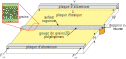
\includegraphics[scale=1]{../Figures_chap_etat/geller.pdf}
\caption[Dispositif expérimental d'étude d'une interface granulaire]{Exemple de dispositif utilisé pour coupler l'élasticité de blocs solides avec une interface granulaire (adapté de\,\cite{geller_stick-slip_2015}). Les grains polydisperses sont pressés et cisaillés à vitesse constante. La géométrie des plaques et des grains est choisie afin de permettre de considérer le système comme bidimensionnel ($H\ll L,W$).}
\label{fig:geller}
\end{figure}


Nous nous intéressons dans notre étude à des interfaces granulaires cisaillées par des solides élastiques. Ces systèmes permettent d'étudier le couplage entre l'élasticité des blocs et la dynamique du milieu granulaire, mais également de considérer que le milieu granulaire est une perturbation d'une interface solide-solide élastique (Fig.\,\ref{fig:geller}).

Le cisaillement par des blocs élastiques d'un milieu granulaire peut mener à une grande diversité de comportements. Il a été montré qu'un tel système peut avoir un mouvement de stick-slip mais également des phases de glissement permanent. Geller et al. montrent que le glissement des deux blocs séparés par un milieu granulaire épais est un glissement lent ponctué par des évènements rapides de chutes de force cisaillante\,\cite{geller_stick-slip_2015}. La distribution de ces chutes de force suit une loi de puissance type Gutenberg-Richter. L'expérience de Geller et al. est très similaire à des systèmes simulés tels que celui présenté par Zhang et al.\,\cite{zhang_two_2023}, qui s'en inspire. Les simulations numériques montrent un bon accord avec les expériences en laboratoire.

Lorsque le milieu granulaire est moins épais, ou évolue avec le temps, il peut perdre progressivement son homogénéité. Cebry et al.\,\cite{cebry_creep_2022} présentent par exemple un système dans lequel une gouge fine de quartz est cisaillée par deux blocs de PMMA. La gouge initialement homogène crée deux points de compressions de part et d'autre de l'interface. La dynamique de l'interface évolue alors au fil du cisaillement d'un glissement lent à une instabilité de stick-slip relativement régulière, puis à un comportement de plus en plus erratique. Cette étude soulève l'importance de l'usure de l'interface. D'autres expériences similaires montrent que l'interface, broyant la poudre qu'elle contient, se lubrifie par son usure dans un phénomène de lubrification solide\,\cite{reches_fault_2010}. Similairement au cas d'une interface solide-solide, des expériences et simulation ont montré que l'initiation du glissement s'accompagne de la propagation d'une rupture à l'interface\,\cite{cebry_creep_2022,buijze_nucleation_2020,buijze_effects_2021}. Cette rupture n'a cependant pas fait l'objet de caractérisations approfondies.
%et n'est a priori pas décrite par les loi de la mécanique de la fracture linéaire élastique.



\section{Objectifs de cette thèse}


Les objectifs de cette thèse sont tout d'abord de développer un dispositif expérimental complet pour notre étude. Ce dispositif doit permettre de presser et cisailler des plaques minces de PMMA encapsulant un milieu granulaire (Chap.\,\ref{sec:chapxp}). En particulier nous souhaitons implémenter des méthodes d'acquisition électronique pour la mesure du tenseur des déformations à haute fréquence permettant d'étudier la propagation de ruptures à l'interface (Sec.\,\ref{sec:electronique}); et des mesures par imagerie pour le suivi des grains (Sec.\,\ref{sec:optique}). Ce dispositif sera ensuite utilisé afin d'analyser la dynamique de plusieurs interfaces frictionnelles complexes incorporant des milieux granulaires. En particulier nous avons pour objectif l'étude d'une interface en œil granulaire (Chap.\,\ref{sec:chaparticle}), et d'une interface entièrement granulaire (Sec.\,\ref{sec:fullygranpersp}).


Par l'étude de ces interfaces nous voulons éclaircir les mécanismes de la friction granulaire à l'échelle microscopique. Pour ce faire nous souhaitons tout d'abord évaluer les modifications de la dynamique du système dues à la présence d'un milieu granulaire, notamment sur le mouvement de stick-slip à l'interface. Nous pourrons ensuite déterminer les mécanismes locaux responsables de ces modifications.

Dans le cas de l'œil granulaire nous nous intéressons en particulier au rôle d'un patch granulaire à l'interface dans la dynamique de glissement et sur l'initiation de ruptures frictionnelles. Les propriétés de cette interface la rapprochent de systèmes de failles de composition hétérogène. Nous espérons par cette étude améliorer la compréhension du couplage entre les portions glissantes et les segments bloqués au sein d'une faille. Dans le cas de l'interface entièrement granulaire, nous avons pour objectif d'étudier l'initiation du mouvement de glissement rapide à l'interface, et avons pour hypothèse qu'elle est médiée par la nucléation et la propagation d'une rupture frictionnelle dans le milieu granulaire. Cette étude permettra une meilleure compréhension du rôle de la gouge de faille dans les mécanismes sismiques.




En résumé, notre étude porte sur les interfaces frictionnelles perturbées par un milieu granulaire. En particulier nous nous intéressons à une interface bidimensionnelle en cisaillement, contenant des grains soit dans toute sa longueur, se rapprochant alors du dispositif expérimental présenté Figure\,\ref{fig:geller}, soit dans un espace restreint rendant l'interface hétérogène, comme présenté en Section\,\ref{sec:hetero}. Elle s'inscrit dans la continuité de l'étude des interfaces frictionnelles solide-solide et de la description de l'initiation du mouvement par la propagation d'une rupture, et vise à déterminer la robustesse de cette description à des perturbations telles que l'inclusion d'un milieu granulaire.

















